
\begin{figure*}[tbh]
\begin{center}
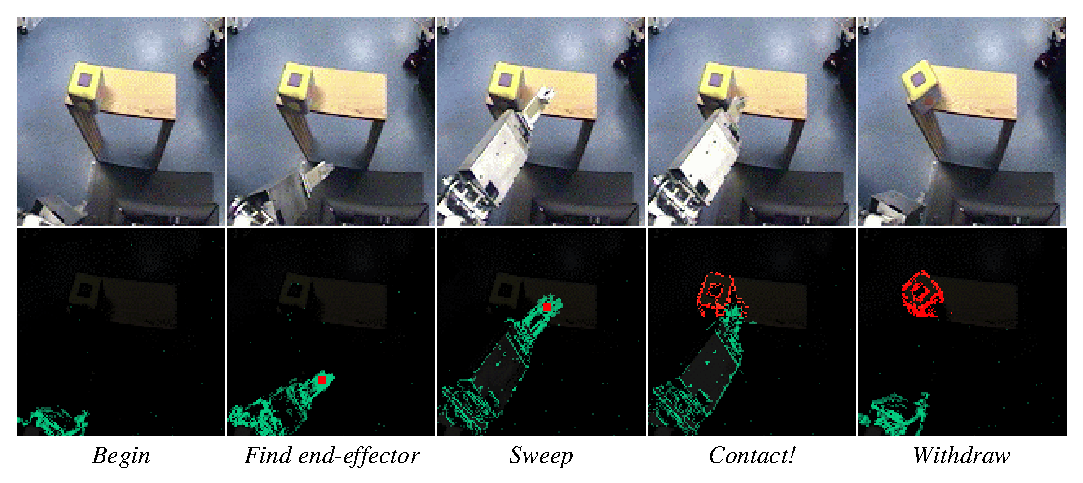
\includegraphics[width=\textwidth]{poking-sequence.eps}
%%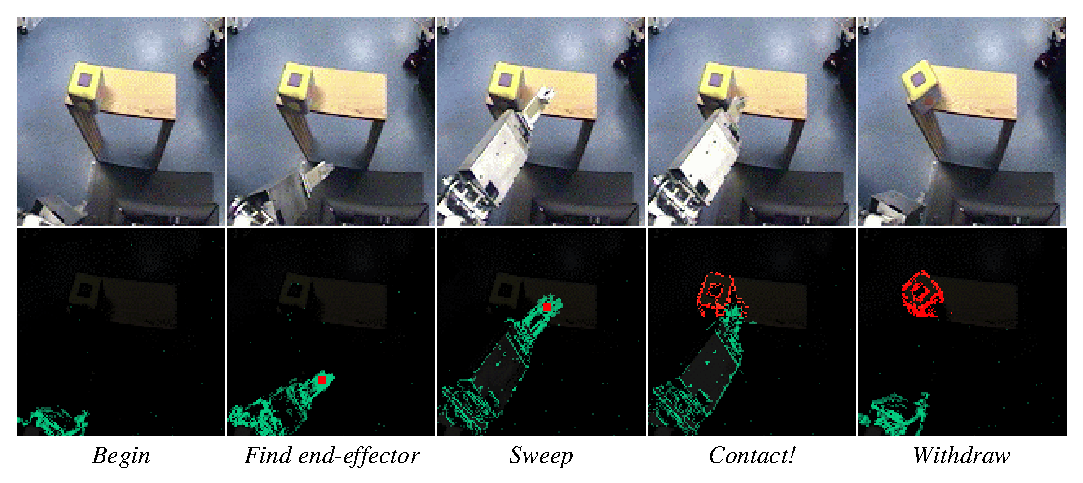
\includegraphics[width=14cm]{poking-sequence.eps}
\caption{ 
\label{fig:poking-sequence}
%
  The upper sequence shows an arm extending into a workspace, tapping
  an object, and retracting.  This is an exploratory mechanism for
  finding the boundaries of objects, and essentially requires the arm
  to collide with objects under normal operation, rather than as an
  occasional accident.  The lower sequence shows the shape
  identified from the tap using simple image differencing and flipper
  tracking.
%
}
\end{center}
\end{figure*}


\section{Perceiving indirect effects of action}
\label{sec:poking}

We have assumed that the target of a reaching operation is chosen
visually.  As discussed in the introduction, visual
segmentation is not easy, so we should not expect a target selected in
\ifrev
this way to be correctly segmented.  For the example scene in
\else
this way to be a correctly segmented.  For the example scene in
\fi
%%Figure~\ref{fig:setup-sequence} 
Figure~\ref{fig:number-cross} 
(a cube sitting on a table), the small
inner square on the cube's surface pattern might be selected as a
target.  The robot can certainly reach towards this target, but
grasping it would prove difficult without a correct estimate of the
object's physical extent.  In this section, we develop a procedure
for refining the segmentation using the same idea of correlated
motion used earlier to detect the arm.

When the arm enters into contact with an object, one of several
outcomes are possible.  If the object is large, heavy, or otherwise
unyielding, motion of the arm may simply be resisted without any
visible effect.  Such objects can simply be ignored, since the robot
will not be able to manipulate them.  But if the object is smaller, it
is likely to move a little in response to the nudge of the arm.  This
movement will be temporally correlated with the time of impact, and
will be connected spatially to the end-effector -- constraints that
are not available in passive scenarios~\cite{birchfield99depth}.  If
the object is reasonably rigid, and the movement has some component in
parallel to the image plane, the result is likely to be a flow field
whose extent coincides with the physical boundaries of the object.



\begin{figure}[tbh]
  \centerline{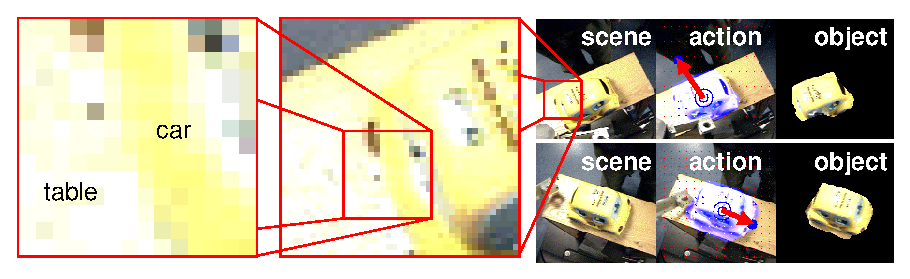
\includegraphics[width=\textwidth]{fig-double-yellow}}
  \label{fig:poking-zoom}
  \caption{
%
An example of the power of active segmentation.  The images
marked ``scene'' show two presentations of a yellow toy car
sitting on a yellow table.  The robot extends its arm across
the table.  In the upper sequence it strikes from below, in the
lower sequence it strikes from the side (``action'' images).
Once the arm comes in contact with the car, it begins to move,
and it can be segmented from the stationary background (``object'').
On the left of the figure, a zoomed view of the car/table
boundary is shown -- the difference between the two is very subtle.
%
} 
\end{figure}


\ifverbose
%
\begin{figure}[tb]
\begin{center}
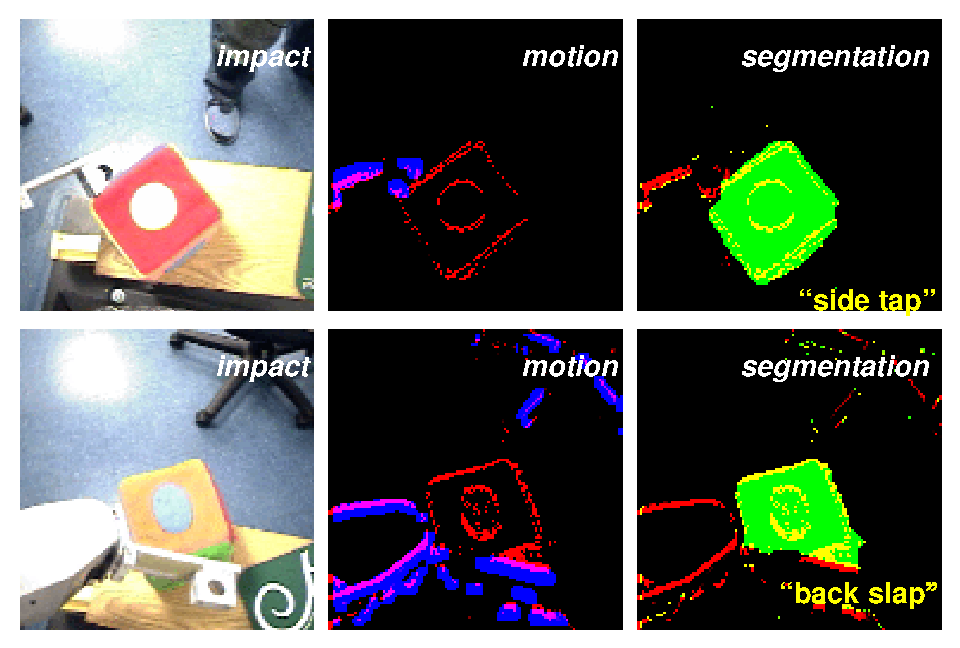
\includegraphics[width=12cm]{segmentation-detail.eps}
\caption{ 
\label{fig:poking-segmentation}
%
Cog batting a cube around.  The top two rows show the flipper poking
the object repeatedly from the side, turning it slightly.  The third
row shows Cog batting an object away.  The images in the first column
are frames prior to a collision.  The second column shows the actual
impact.  The third column shows the motion signal at the point of
contact.  The bright regions in the images in the final column show
the segmentations produced for the object. 
%
}
\end{center}
\end{figure}
%
\fi

Figure~\ref{fig:poking-sequence} shows how a ``poking'' movement can
be used to refine a target.  During a poke operation, the arm begins
by extending outwards from the resting position.  The end-effector (or
``flipper'') is localized as the arm sweeps rapidly outwards, using
the heuristic that it lies at the highest point of the region of optic
flow swept out by the arm in the image (the head orientation and
reaching trajectory are controlled so that this is true).  The arm is
driven outward into the neighborhood of the target which we wish to
define, stopping if an unexpected obstruction is reached.  If no
obstruction is met, the flipper makes a gentle sweep of the area
around the target.  This minimizes the opportunity for the motion of
the arm itself to cause confusion; the motion of the flipper is
bounded around the endpoint whose location we know from tracking
during the extension phase, and can be subtracted easily.  Flow not
connected to the end-effector can be ignored as a distractor.  
For simplicity, the head is kept steady throughout the poking
operation, so that simple image differencing can be used to detect
the presence of motion at a higher resolution than optic flow.
Figure~\ref{fig:poking-zoom} shows an example of the kind of 
results that are possible (see Section~\ref{sect:recognition} for 
further examples).

%Because a poking
%operation currently always starts from the same location, the arm
%is localized using a simple heuristic rather than the procedure described
%in the previous section -- the first region of optic flow appearing
%in the lower part of the robot's view when the reach begins
%is assumed to be the arm.

\ifverbose
\begin{figure}[tbh]
\begin{center}
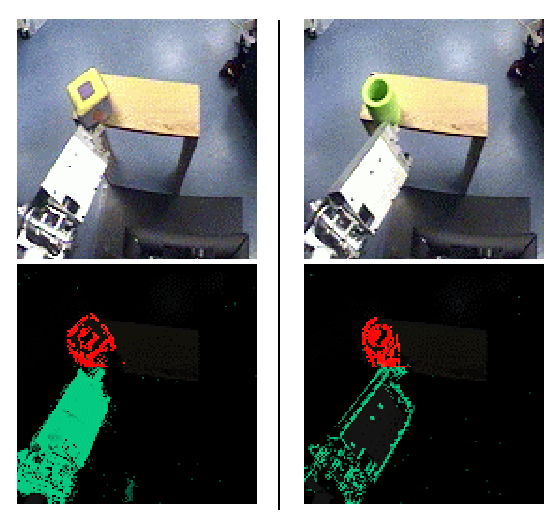
\includegraphics[width=\columnwidth]{cube-and-cylinder.eps}
\caption{ 
\label{fig:cube-and-cylinder}
%
  Poking can reveal a diffence in the shape of two objects without
  any prior knowledge of their appearance.
%
}
\end{center}
\end{figure}
\fi

The poking operation gives clear results for a rigid object that is
free to move.  What happens for non-rigid objects and objects that are
attached to other objects?  Here the results of poking are likely to
be more complicated to interpret -- but in a sense this is a good
sign, since it is in just such cases that the idea of an object
becomes less well-defined.  Poking has the potential to offer an
operational theory of ``objecthood'' that is more tractable than a
vision-only approach might give, and which cleaves better to the true
nature of physical assemblages.  The idea of a physical object is
rarely completely coherent, since it depends on where you draw its
boundary and that may well be task-dependent.  Poking allows us to
determine the boundary around a mass that moves together when
disturbed, which is exactly what we need to know for manipulation.  As
an operational definition of object, this has the attractive property
of breaking down into ambiguity in the right circumstances -- such
as for large interconnected messes, floppy formless ones, liquids,
and so on.


\ifverbose

\section{Active Segmentation}

Gives a sketch of the min-cut algorithm and how it is applied to
this domain.

\begin{figure*}[tbh]
\begin{center}
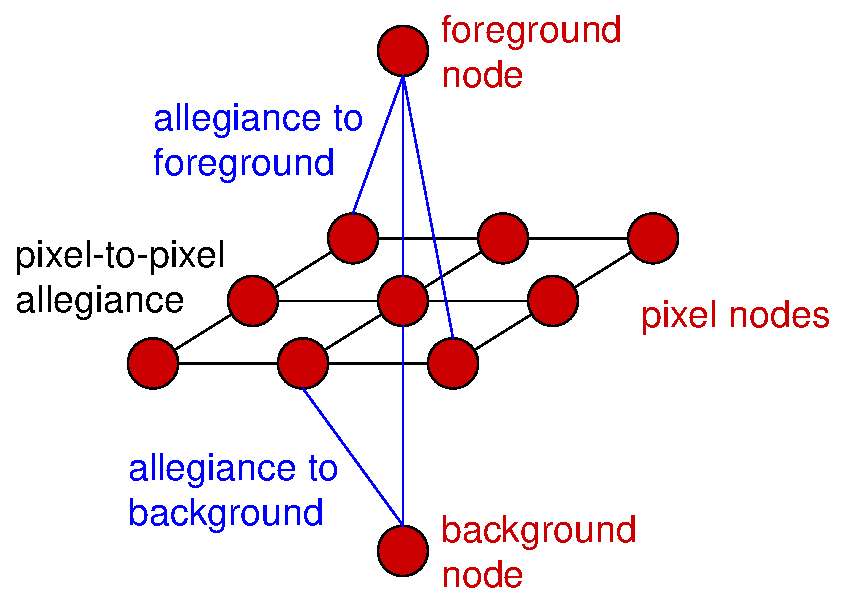
\includegraphics[width=7cm]{cut-graph1.eps}
\hspace{1cm}
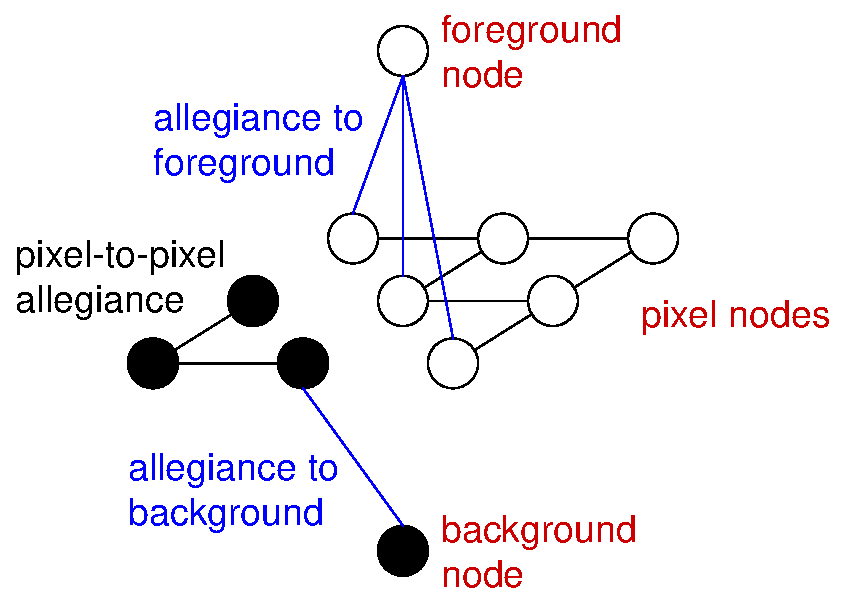
\includegraphics[width=7cm]{cut-graph2.eps}
\caption{ 
\label{fig:cut-graph}
%
A simple example of the graph cut algorithm in operation.  
The left graph represents the output of the point-of-contact 
processing.  Edges in the graphs are weighted by how much
it will cost to split connected nodes.  The bulk of the nodes
are in one-to-one correspondence with pixels in the image.
There are two extra nodes corresponding to the foreground and
background.  The goal is to split the graph into two by removing
edges.  The cost of the split is the sum of the weights on the 
edges removed.  There are good approximate algorithms for
finding a minimum cost solution [ref].
%
}
\end{center}
\end{figure*}

Use 16-connectivity (8 neighbors, plus cells connected by a
``knight'' move).

%
\begin{figure}[tb]
\begin{center}
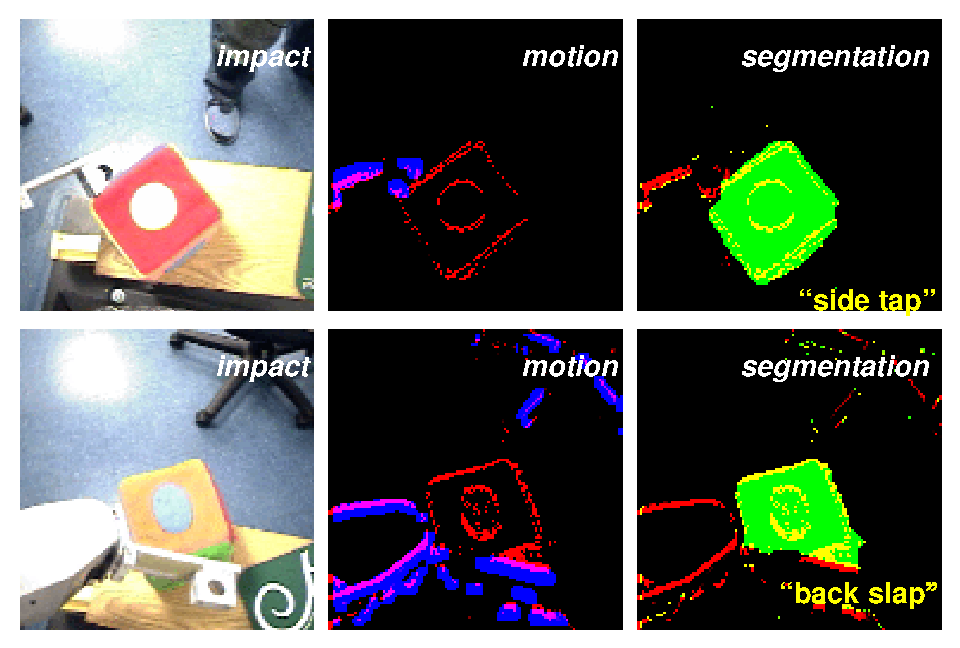
\includegraphics[width=\columnwidth]{segmentation-detail.eps}
\caption{ 
\label{fig:poking-segmentation}
%
Cog batting a cube around.  The top two rows show the flipper poking
the object repeatedly from the side, turning it slightly.  The third
row shows Cog batting an object away.  The images in the first column
are frames prior to a collision.  The second column shows the actual
impact.  The third column shows the motion signal at the point of
contact.  The bright regions in the images in the final column show
the segmentations produced for the object. 
%
}
\end{center}
\end{figure}
%

\begin{figure}[tbh]
  \centerline{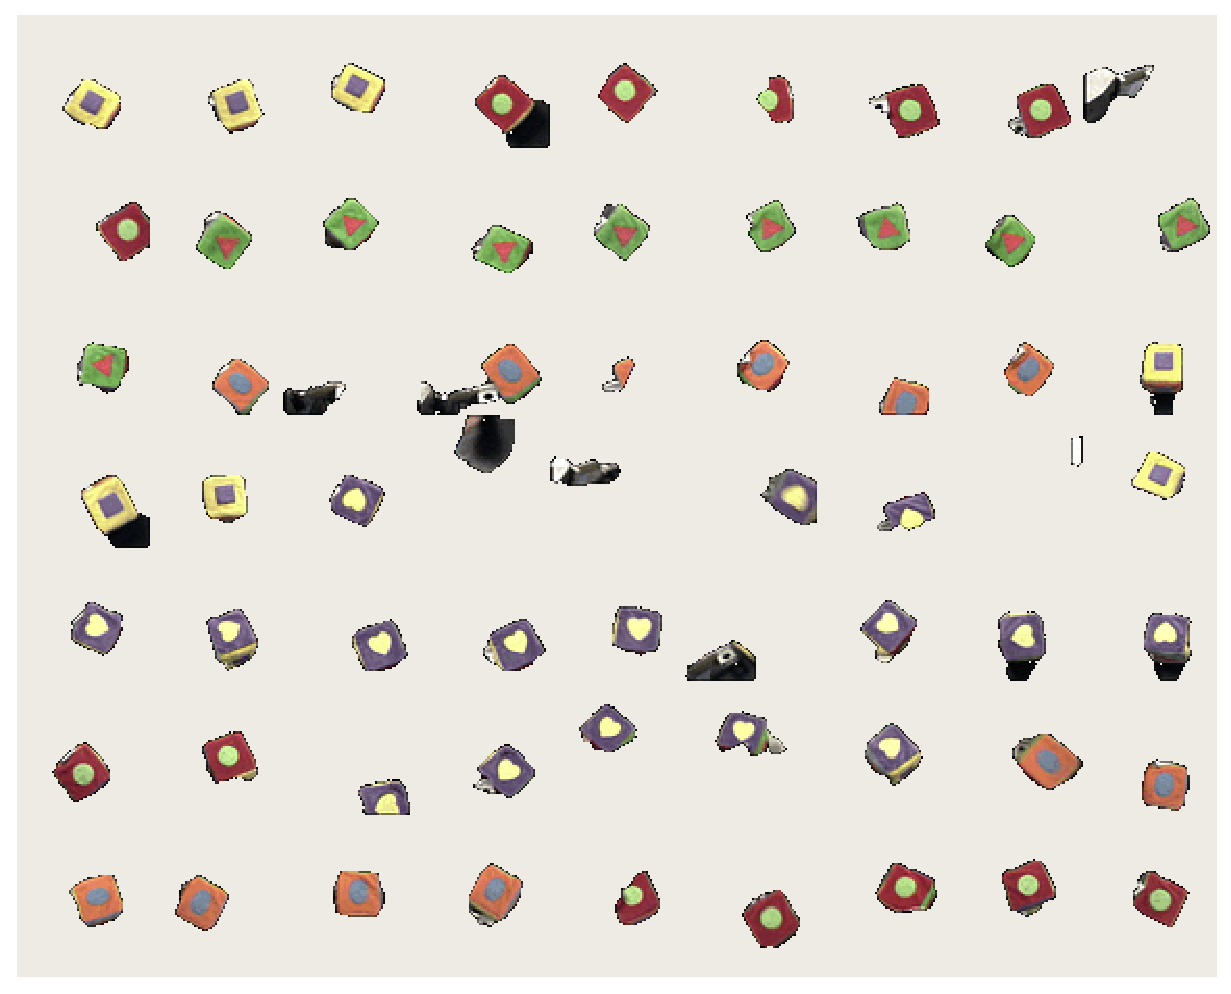
\includegraphics[width=2.5in]{experiment-montage}}
  \caption{Sample results}
  \label{fig:sample-results}
\end{figure}



\section{Detecting the point of collision}

Two components -- detecting the moment of impact, and extracting as 
much data as possible from the frames around it.

There are particular periods when the robot is attentive and fixating.
When this is so, it can detect visually when a collision occurs
between a moving object and a previously stationary object in view.
The principal task, then, is keep the motion of the moving object distinct
from that of the impacted object.

Brief introduction to image differencing and background subtraction.
Stationary camera assumption to facilitate pixel modeling.  Don't want
to keep head stationary, but can fixate for significant periods.

Image differencing is a very simple technique for detecting motion by
simply subtracting successive frames from a camera and looking for
pixel-level differences.  A moving object that has some contrast with
the background it is moving over will generate such differences.  Of
course, pixel differences can also be generated by changes in
illumination, cast shadows, computer monitors, movement of the camera
itself, etc.  A related technique called background modeling tries to
estimate the appearance of the fixed, stationary background of a 
scene, and then subtract the current view from the reference to 
detect new foreground.  While these techniques are not ideally
suited to a moving platform like our robot, they are short periods 
during which they can be useful.  In particular, when the robot is
fixating a target, we can do this.

Within the context of the robot fixating a target, we try to detect
the moment of impact precisely, so we can apply the (relatively) slow
segmentation optimization to a narrow interval of the video input and
maintain close to real-time performance.  A moving manipulator
colliding with an object will accelerate it, if it is not too massive.
If the object is rigid, the motion of the manipulator will be transmitted 
through it.  This transmission can be detected as a spreading motion
that is not plausibly generated by the manipulator itself.

Some assumptions that may fail: object not too heavy; object at least
semi-rigid; manipulator not moving above a certain speed; manipulator
not casting shadows on the object itself.  When the robot is poking the
object itself, it can control some of this.  If the object iself is
troublesome, then we potentially diagnose this, or just ignore it.

%%We are relying on some facts about optic flow.  When an object is ...

\begin{figure}[tbh]
  \begin{center}
    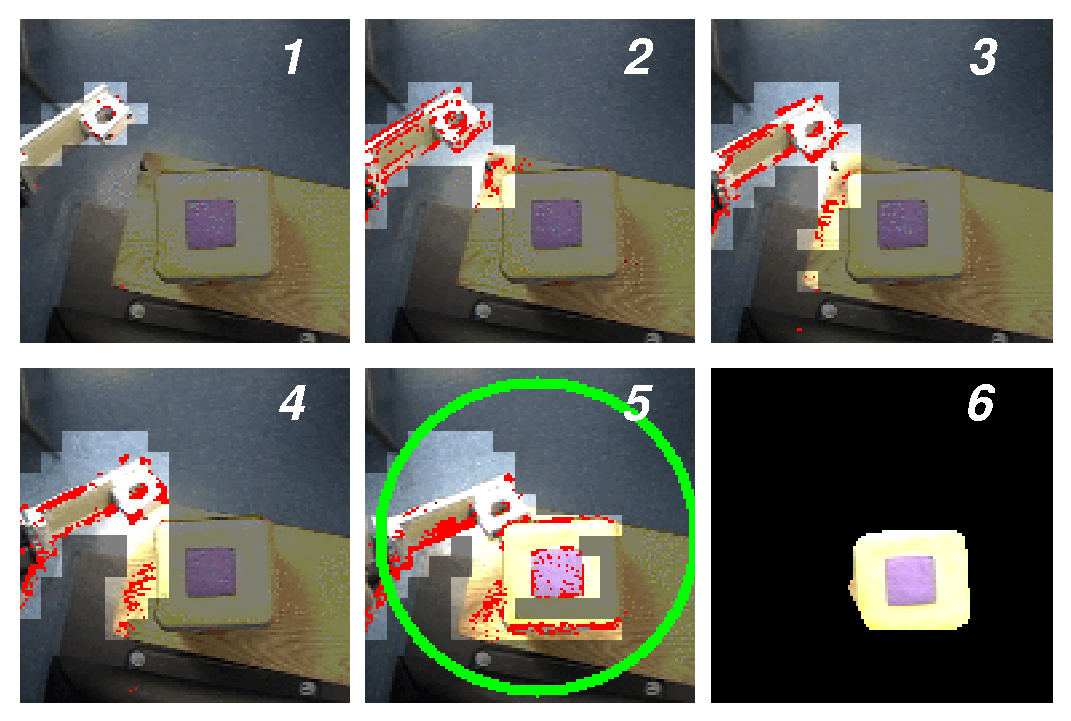
\includegraphics[width=12cm]{collision-detail}
  \end{center}
  \caption{
    The moment of impact is detected visually by the
    sudden expansion of motion away from the arm.  Motion before and
    after contact is compared to gather information for segmentation.
}
\end{figure}


\fi


